\section{The Case for Benchmark Generators}%
\label{sec:the-case-for-benchmark-generators}

This section makes the argument for synthetic benchmarks. Frequently used benchmark suites were identified in a survey of 25 research papers in the field of GPGPU performance tuning from four top tier conferences between 2013--2016: CGO, HiPC, PACT, and PPoPP. The average number of benchmarks used in each paper is 17, and a small pool of benchmarks suites account for the majority of results, illustrated in Figure~\ref{fig:benchmark-suite-distribution}. The performance of the state-of-the-art \emph{Grewe et   al.}~\cite{Grewe2013} predictive model was evaluated across each of the 7 most frequently used benchmark suites (accounting for 92\% of results in the surveyed papers). The \emph{Grewe et   al.}~model predicts whether running a given OpenCL kernel on the GPU gives better performance than on the CPU. The full experimental setup is described in Section~\ref{sec:clgen-eval-methodology}.

\begin{figure}
	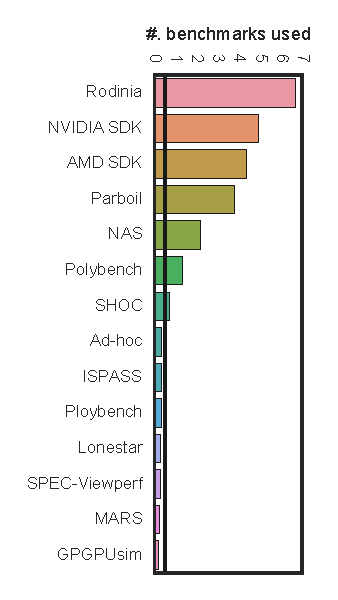
\includegraphics[width=\columnwidth]{img/motivation-c} %
	\caption[Benchmark counts in GPGPU research papers]{%
		The average number of benchmarks used in GPGPU research papers published between 2013-2016 in CGO, HiPC, PACT, and PPoPP conferences.%
	}%
	\label{fig:benchmark-suite-distribution}
\end{figure}

Table~\ref{tab:cpu-gpu-benchmarks-crossvalidate} summarises the results. The performance of a model trained on one benchmark suite and used to predict the mapping for another suite is generally very poor. The benchmark suite which provides the best results, NVIDIA SDK, achieves on average only 49\% of the optimal performance. The worst case is when training with Parboil to predict the optimal mappings for Polybench, where the model achieves only 11.5\% of the optimal performance. From this it is clear that heuristics learned on one benchmark suite fail to generalise across other suites.

\begin{table}
	\centering
	\rowcolors{2}{gray!25}{white}
\begin{tabular}{ | R{2.0cm} | C{1.25cm} C{1.25cm} C{1.25cm} C{1.25cm} C{1.25cm} C{1.25cm} C{1.25cm} | }
  \hline
  \rowcolor{gray!50}
  & \rotatebox[origin=c]{90}{\textbf{AMD}} & \rotatebox[origin=c]{90}{\textbf{NPB}} & \rotatebox[origin=c]{90}{\textbf{NVIDIA}} & \rotatebox[origin=c]{90}{\textbf{Parboil}} & \rotatebox[origin=c]{90}{\textbf{Polybench}} & \rotatebox[origin=c]{90}{\textbf{Rodinia}} & \rotatebox[origin=c]{90}{\textbf{SHOC}}\\
  \hline
  \textbf{AMD} & - & 38.0\% & 74.5\% & 76.7\% & 21.7\% & 45.8\% & 35.9\%\\
  \textbf{NPB} & 22.7\% & - & 45.3\% & 36.7\% & 13.4\% & 16.1\% & 23.7\%\\
  \textbf{NVIDIA} & 29.9\% & 37.9\% & - & 21.8\% & 78.3\% & 18.1\% & 63.2\%\\
  \textbf{Parboil} & 89.2\% & 28.2\% & 28.2\% & - & 41.3\% & 73.0\% & 33.8\%\\
  \textbf{Polybench} & 58.6\% & 30.8\% & 45.3\% & 11.5\% & - & 43.9\% & 12.1\%\\
  \textbf{Rodinia} & 39.8\% & 36.4\% & 29.7\% & 36.5\% & 46.1\% & - & 59.9\%\\
  \textbf{SHOC} & 42.9\% & 71.5\% & 74.1\% & 41.4\% & 35.7\% & 81.0\% & -\\
  \hline
\end{tabular}

  \caption[Cross-validation of benchmark suites on a predictive model]{%
    Performance relative to the optimal of the \emph{Grewe et al.\ }predictive model across different benchmark suites on an AMD GPU. The columns show the suite used for training; the rows show the suite used for testing.%
  }
  \label{tab:cpu-gpu-benchmarks-crossvalidate}
\end{table}

This problem is caused both by the limited number of benchmarks contained in each suite, and the distribution of benchmarks within the feature space. Figure~\ref{fig:pca-benchmarks} shows the feature space of the Parboil benchmark suite, showing whether, for each benchmark, the model was able to correctly predict the appropriate optimisation. Principle Component Analysis is used to reduce the multi-dimensional feature space to aid visualisation.

\begin{figure}
	\centering
	\subfloat{%
		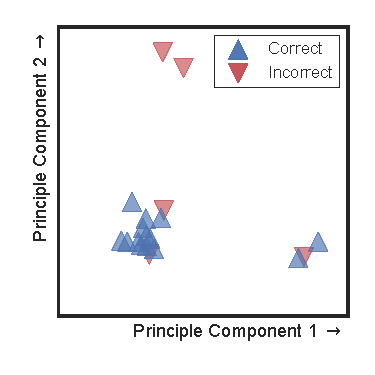
\includegraphics[width=.55\columnwidth]{img/motivation-a}%
		\label{fig:pca-benchmarks-a}%
	}%
  \\*
	\subfloat{%
		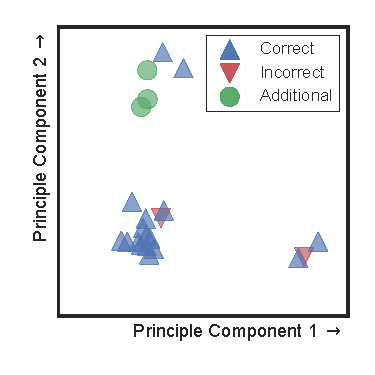
\includegraphics[width=.55\columnwidth]{img/motivation-b}%
		\label{fig:pca-benchmarks-b}%
	}%
	\caption[Identifying and correcting outliers in a benchmark suite]{%
    A two dimensional projection of the \emph{Grewe et al.\ }feature space, showing predictive model results over Parboil benchmarks on an NVIDIA GPU. Two outliers in~\protect\subref{fig:pca-benchmarks-a} are incorrectly predicted due to the lack of nearby observations. The addition of neighbouring observations in~\protect\subref{fig:pca-benchmarks-b} corrects this.%
  }%
	\label{fig:pca-benchmarks}
\end{figure}

As can be seen in Figure~\ref{fig:pca-benchmarks-a}, there is a dense cluster of neighbouring benchmarks, a smaller cluster of three benchmarks, and two outliers. The lack of neighbouring observations means that the model is unable to learn a good heuristic for the two outliers, which leads to them being incorrectly optimised. In Figure~\ref{fig:pca-benchmarks-b}, I hand-selected benchmarks which are neighbouring in the feature space and retrained the model. The addition of these observations (and the information they provide about that part of the feature space) causes the two outliers to be correctly optimised. Such outliers can be found in all of the benchmark suites of Table~\ref{tab:cpu-gpu-benchmarks-crossvalidate}.

These results highlight the significant effect that the number and distribution of training programs has on the quality of predictive models. Without good coverage of the feature space, any machine learning methodology is unlikely to produce high quality heuristics, suitable for general use on arbitrary real applications, or even applications from different benchmark suites. The novel approach described in the next section addresses this problem by generating an unbounded number of programs to cover the feature space with fine granularity.
